% -*- root: ../ex6.tex -*-

\section{Modification of given data} % (fold)
\label{sec:modification_of_given_data}
Our solver can solve for different seed functions $f(x,y)$ by doing a small modification in the source code. By changing the function \texttt{source} in \texttt{poisson2D.c} it will populate \textbf{B} with the correct given data before solving the system. If you want to be able to see the error you will also have to change \texttt{exact} so that it will calculate the correct error.

There is a restriction to which seed functions $f(x,y)$ you can use as they have to satisfy the boundary conditions given by $u = 0$ on $\partial\Omega$.

Contour plots of the solution of $\mathbf{B}$ for various $f(x,y)$ is shown in Figure~\ref{fig:contourplots}.


\begin{figure}[htbp]
  \centering
  \begin{subfigure}[b]{0.49\textwidth}
    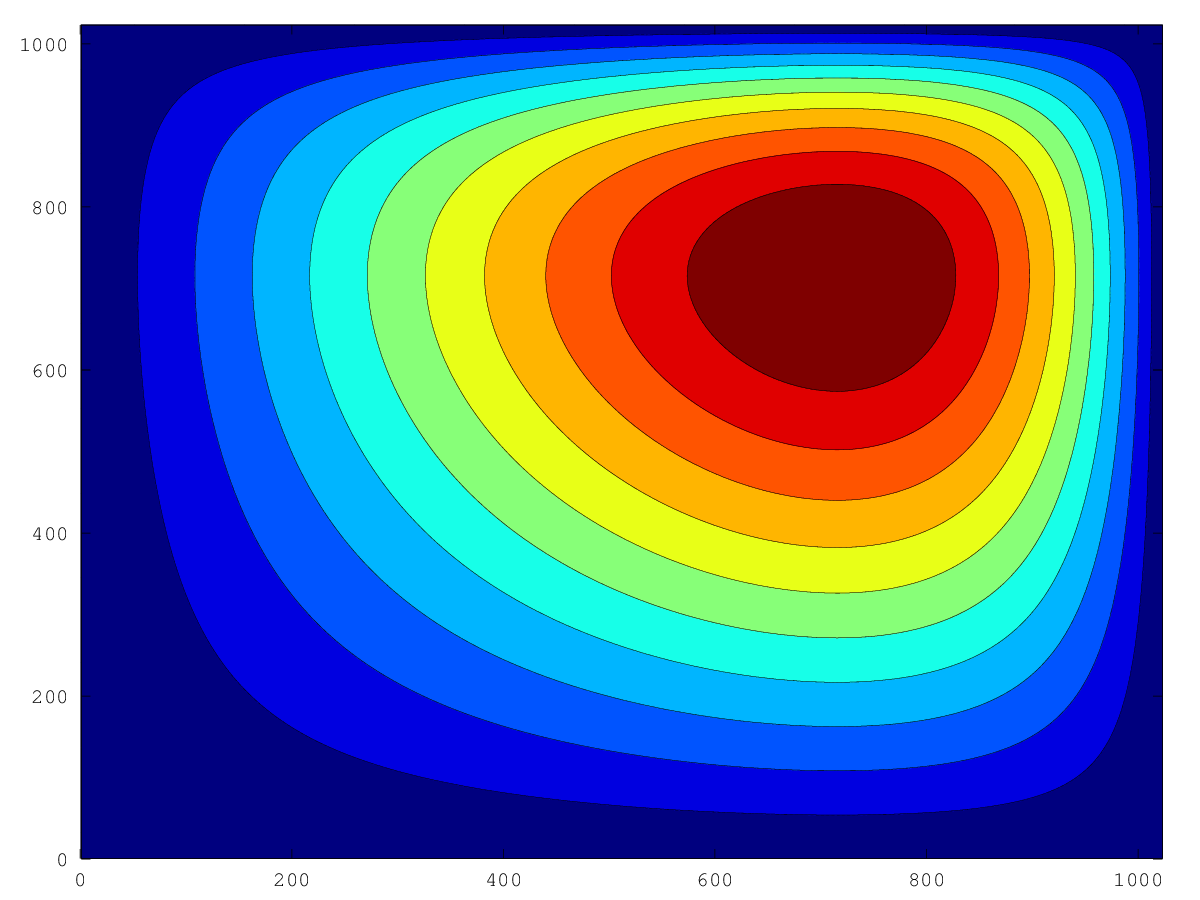
\includegraphics[width=\textwidth]{illustrations/orig.png}
    \caption{$f(x,y) = -30 y^4 x(x^5-1) - 30x^4 y (y^5-1)$}
    \label{fig:contour_1}
  \end{subfigure}
  \begin{subfigure}[b]{0.49\textwidth}
    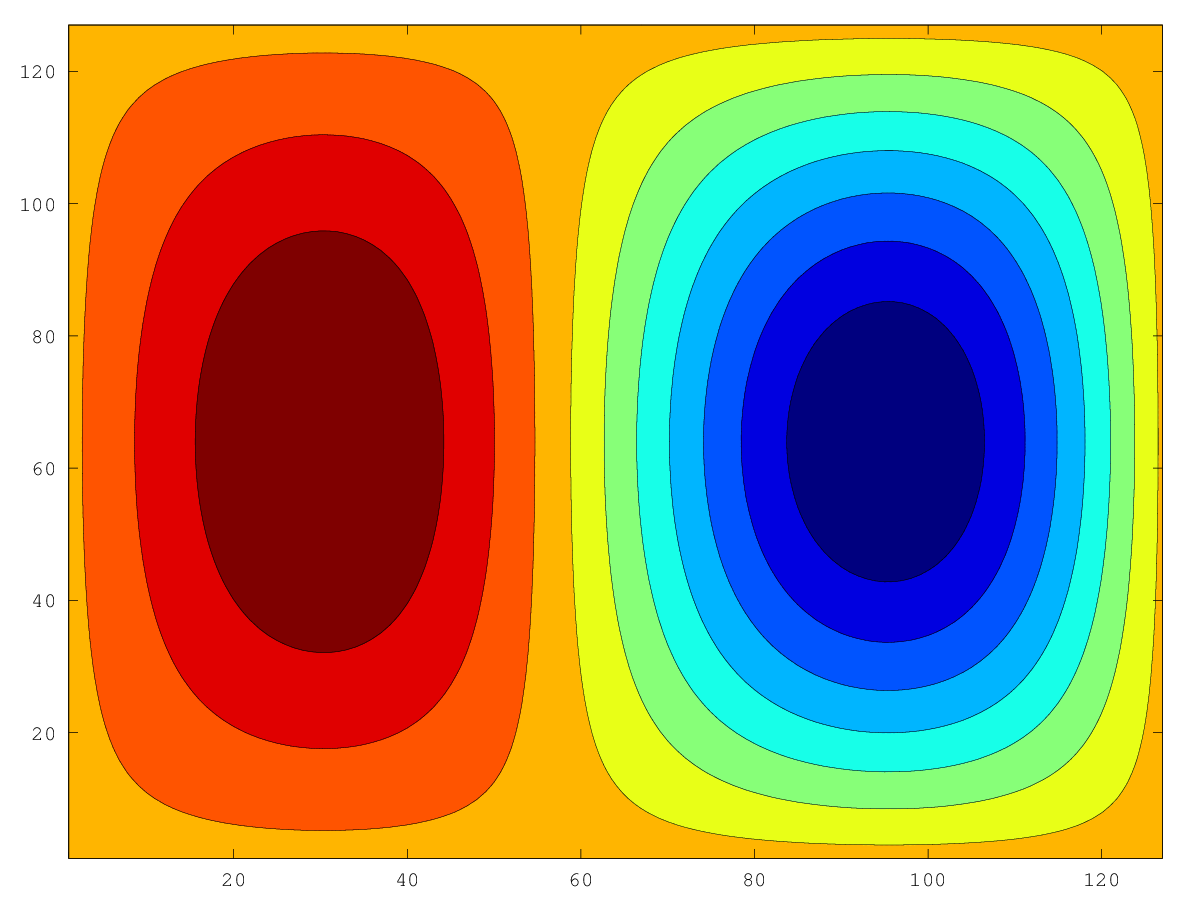
\includegraphics[width=\textwidth]{illustrations/sine.png}
    \caption{$f(x,y) = e^x \times \sin{(2\pi x)} \times \sin{(\pi y)}$}
    \label{fig:contour_2}
  \end{subfigure}

  \medskip

  \begin{subfigure}[b]{0.49\textwidth}
    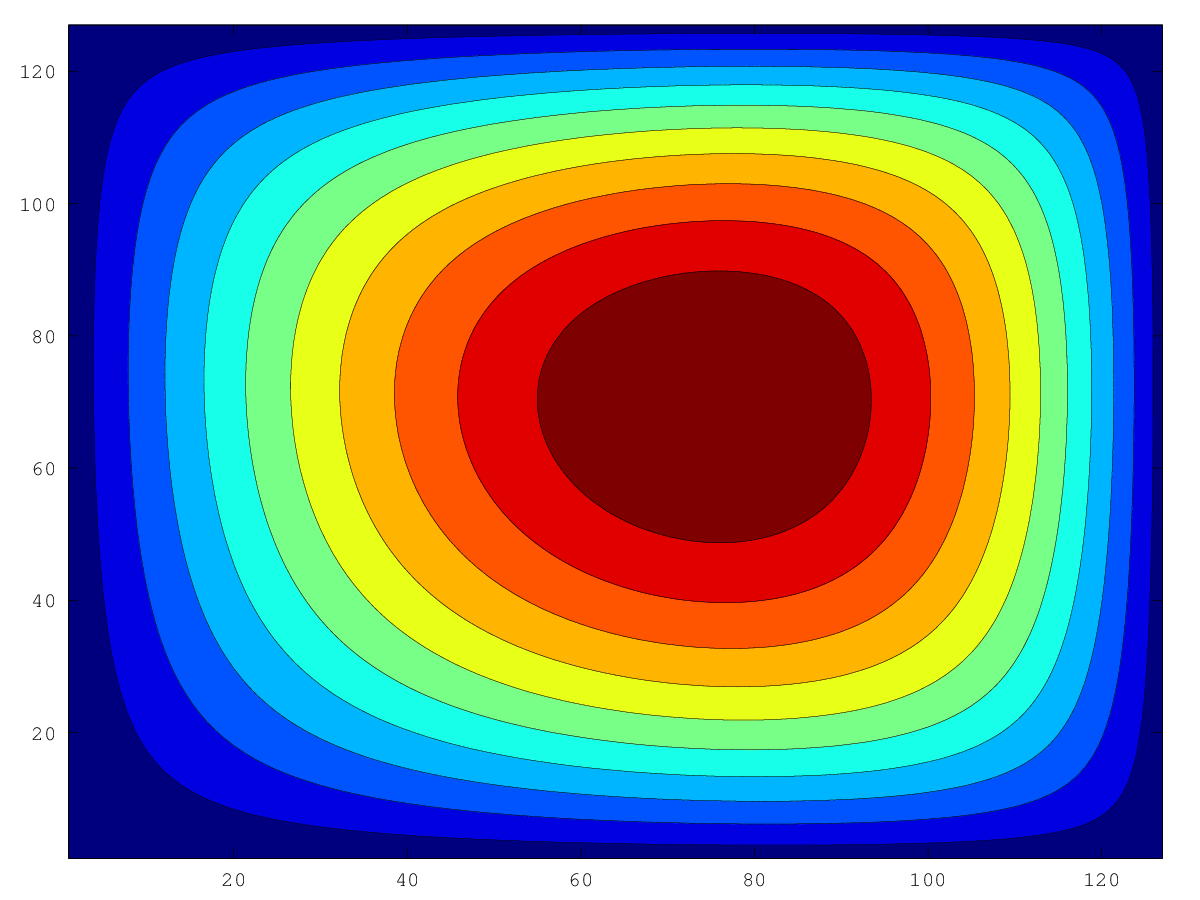
\includegraphics[width=\textwidth]{illustrations/xy.png}
    \caption{$f(x,y) = 2x+y$}
    \label{fig:contour_3}
  \end{subfigure}
  \begin{subfigure}[b]{0.49\textwidth}
    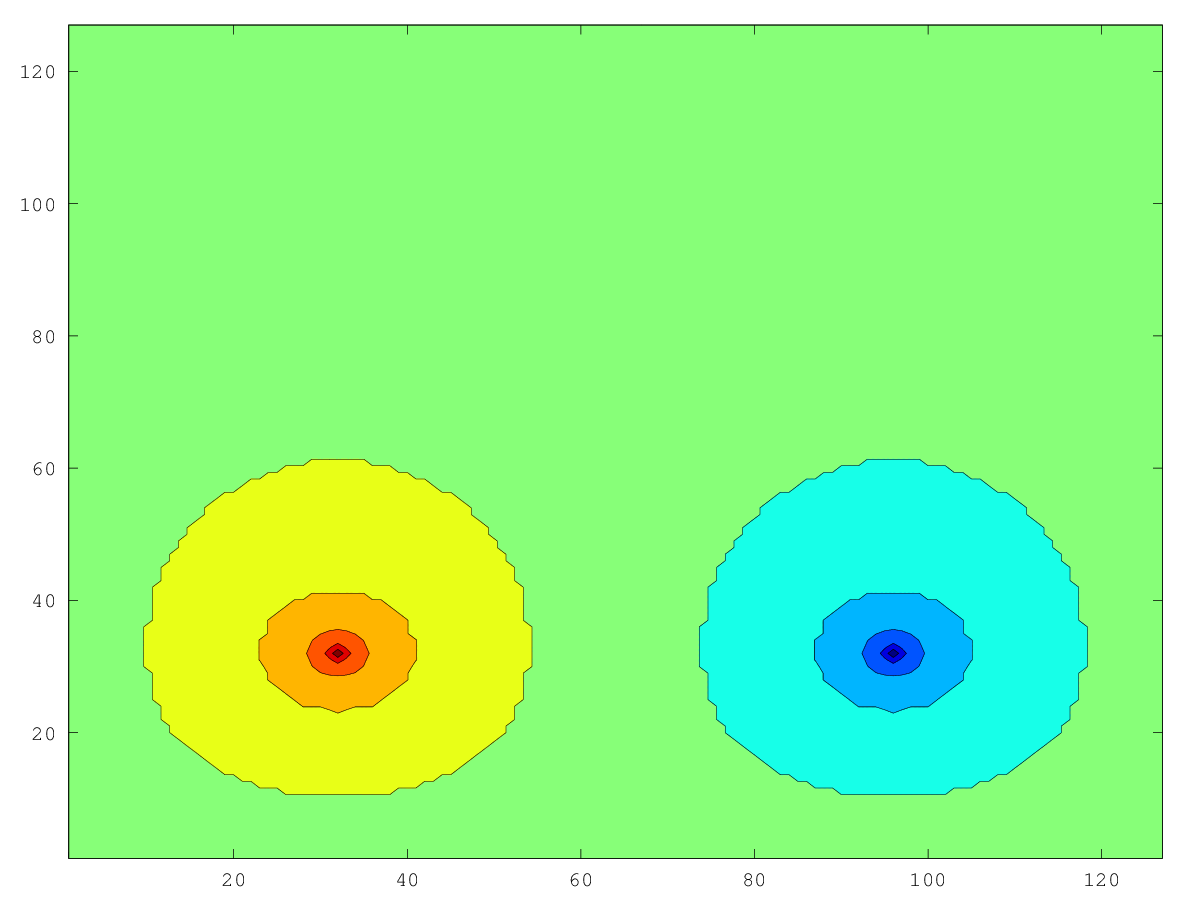
\includegraphics[width=\textwidth]{illustrations/2_points.png}
    \caption{$f(x,y)=0, f(x_1,y_1)=1,f(x_2,y_2)=-1$}
    \label{fig:contour_4}
  \end{subfigure}
  \caption{Contour plots of the solution $\mathbf{B}$ for various $f(x,y)$.}
  \label{fig:contourplots}
\end{figure}

\clearpage

% section modification_of_given_data (end)


% if (x == 0.25 && y == 0.25)
%   //   return 1.0;
%   // else if (x== 0.75 && y == 0.25)
%   //   return -1.0;
%   // else return 0.0;
